\documentclass{article}

\usepackage{geometry}
 \geometry{
 a4paper,
 total={170mm,257mm},
 left=20mm,
 top=20mm,
 }

\setlength{\parskip}{7pt}
\setlength{\parindent}{0pt}

\title{OpenOCD for RISC-V}
\date{2019-10-14}

\PassOptionsToPackage{hyphens}{url}\usepackage{hyperref}
\usepackage{listings}
\usepackage{amssymb}
\usepackage{graphicx}
\graphicspath{ {./images/} }
\usepackage{float}

\lstset{
	breaklines=true,
	columns=fullflexible,
	tabsize=4,
	showstringspaces=false,
	frame=single
}

\begin{document}
	\maketitle
	
	\section{About}
	
	OpenOCD is a software that provides on-chip debugging, in-system programming and boundary-scan testing tools.
	
	The official website is \url{openocd.org}
	
	\begin{figure}[H]
	\centering
	
\includegraphics[width=0.6\textwidth]{openocd.png}
	\end{figure}
	
	A fork with RISC-V support is available on \url{https://github.com/riscv/riscv-openocd}
	
	OpenOCD is free software and is licensed under the \textbf{GNU General Public License v2.0}
	
	This document presents a way of using OpenOCD to debug a RISC-V platform using a JTAG connection.
	
	
	\newpage
	\section{Position in the debug system}
	
	OpenOCD can be used as a translator between GDB and a RISC-V platform, as can be seen in the RISC-V external debug specification.
	
	\begin{figure}[H]
   	\centering
   	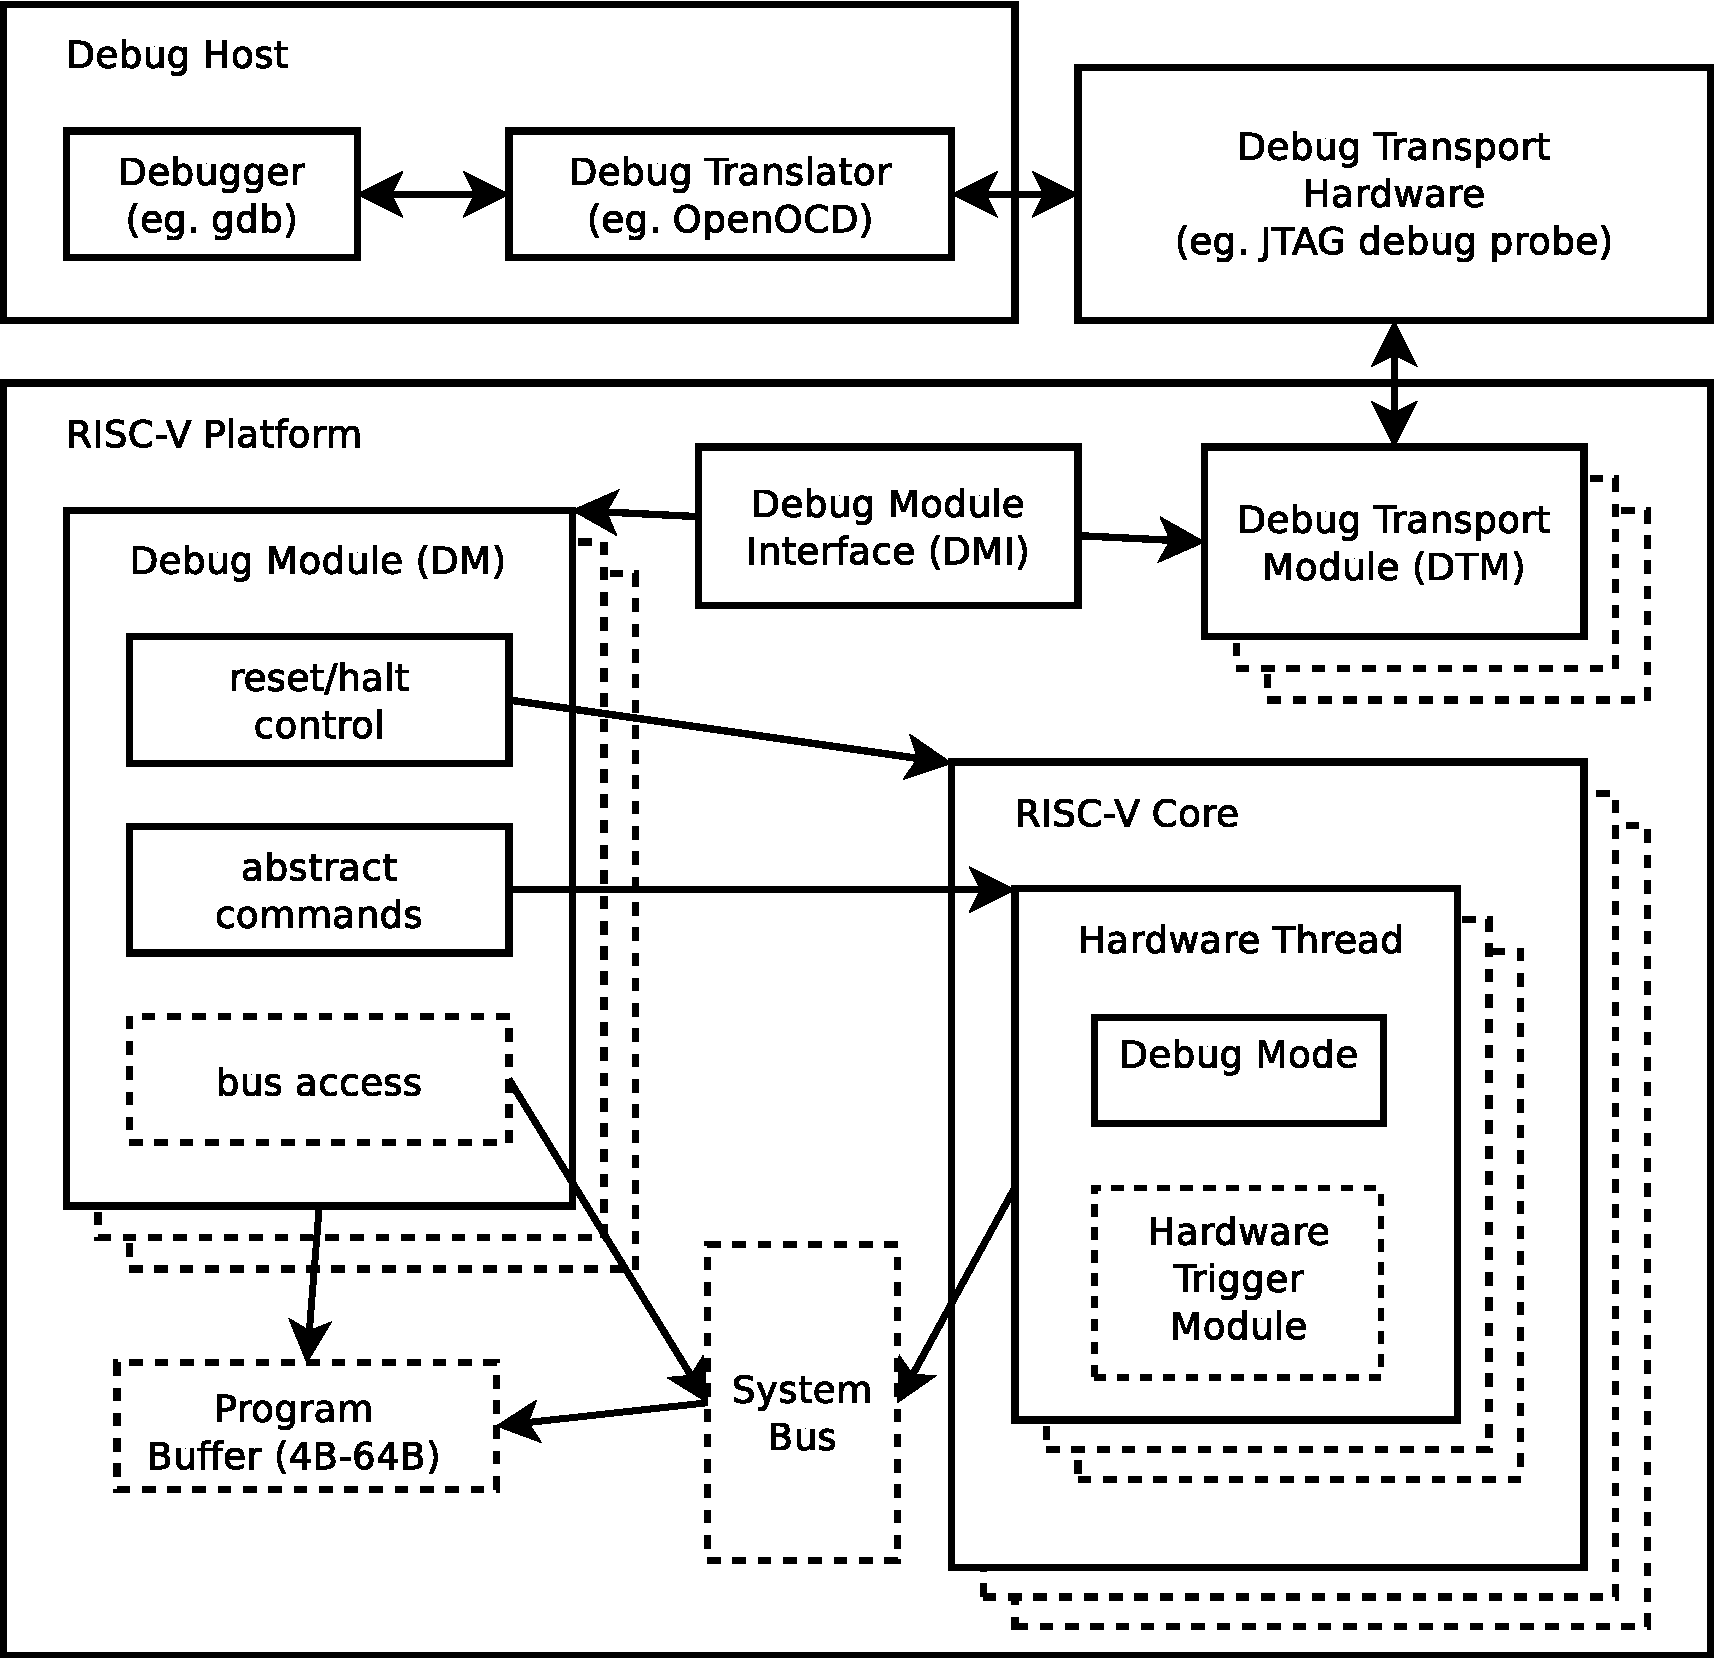
\includegraphics[width=0.82\textwidth]{overview.pdf}
   	\caption{RISC-V Debug System Overview}
   	\label{fig:overview}
	\end{figure}
	
	OpenOCD can connect to GDB in two ways: with a TCP/IP socket or with pipes (stdin/stdout). 
	
	More information here: \url{http://openocd.org/doc-release/html/GDB-and-OpenOCD.html}
	
	A debug adapter is needed to connect OpenOCD to the RISC-V platform. This document focuses on using JTAG transport hardware.
	
	\newpage
	\section{Config file}
	
	\url{http://openocd.org/doc-release/html/OpenOCD-Project-Setup.html}
	
	A typical usage of OpenOCD is:
	
	\begin{lstlisting}[language=bash]
    $ openocd -f config_file.cfg
    \end{lstlisting}
    
    A config file contains commands that OpenOCD will execute using its Jim-Tcl interpreter.
    
    A single file can be broken into several ones. The command line call would then list every file in the correct order:
    
    \begin{lstlisting}[language=bash]
    $ openocd -f config_file_1.cfg config_file_2.cfg config_file_3.cfg
    \end{lstlisting}
    
    It is also possible to launch a single command:
    
    \begin{lstlisting}[language=bash]
    $ openocd -c "a command"
    \end{lstlisting}
    
    \subsection{Interface}
    
    \url{http://openocd.org/doc-release/html/Debug-Adapter-Configuration.html}
    
    The interface configuration tells OpenOCD how to use the transport hardware. 
    
    Config files for a lot of debug adapters can be found where OpenOCD was installed. The path should be \textbf{build/share/openocd/scripts/interface}.
    
    Otherwise, refer to examples and the official documentation.
    
    \subsection{TAP declaration}
    
    \url{http://openocd.org/doc-release/html/TAP-Declaration.html}
    
    A device with a JTAG interface means the device has a Test Access Port (TAP). You need to set up the active TAPs of the device by declaring them inside a configuration file.
    
    Typically, this is achieved in a few lines:
    
    \begin{lstlisting}[language=tcl]
    set _CHIPNAME riscv
    jtag newtap $_CHIPNAME cpu -irlen 5 -expected-id 0x12345678
    \end{lstlisting}
    
    
    
    
	
\end{document}